\section{Problem Statement}
% \subsection{Dominant patterns}
\begin{figure}
\begin{center}
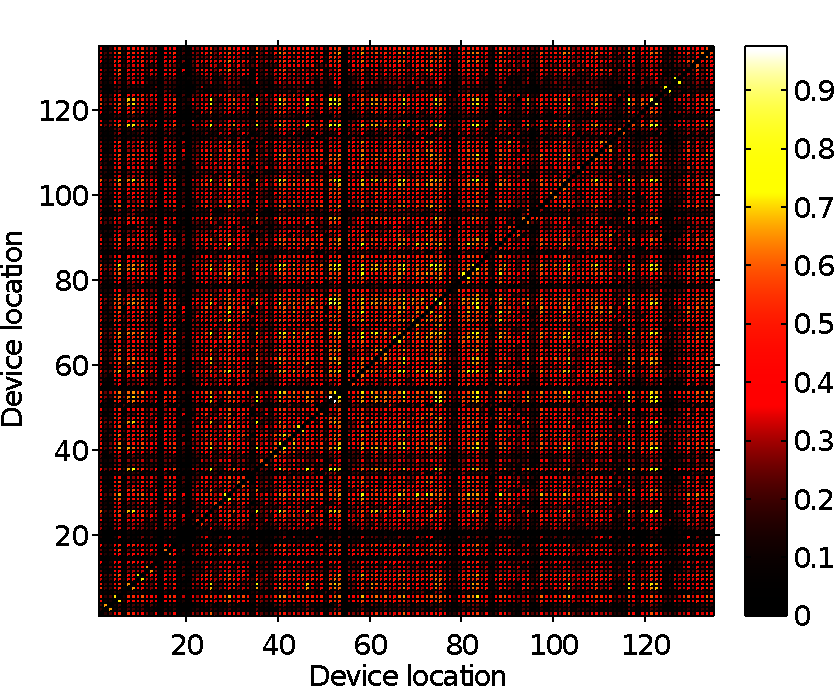
\includegraphics[width=.45\textwidth]{img/heatMap_raw_201106-eps-converted-to.pdf}
\caption{Correlation coefficients of the raw traces from the Engineering Building 2 dataset (Section \ref{data:engbldg2}).
The matrix is ordered such as the devices serving same/adjacent rooms are nearby in the matrix.}
\label{fig:heatmap:raw}
\end{center}
\end{figure}

The first step of the proposed approach is to uncover from the raw data the devices that are used all together.
The basic tool that allows us to compare the devices energy consumption is the correlation coefficient.
However, during our experiments we found that it provides poor help when it is directly applied to the raw signals.
For example the two raw signals of Figure \ref{fig:diagram1} are from two independent HVACs serving distinct rooms on different floors.
Since these devices are independently controlled we expect their signals to be uncorrelated, however, their correlation coefficient (i.e. $0.5675$) indicates the opposite.
Another example with 135 devices is depicted in Figure \ref{fig:heatmap:raw}.
In this correlation matrix the devices indexes are selected such as the devices serving the same or adjacent rooms are also nearby in the matrix.
Thus devices serving the same room are along the diagonal and because they are used simultaneously by the room users we expect them to feature the highest correlation scores.
However, such structure is unseen in the Figure \ref{fig:heatmap:raw}, on the contrary, most of the signals are correlated all together.
% thus this metric prevents us from finding devices that are used in concert.

\begin{figure}[t!]
\begin{center}
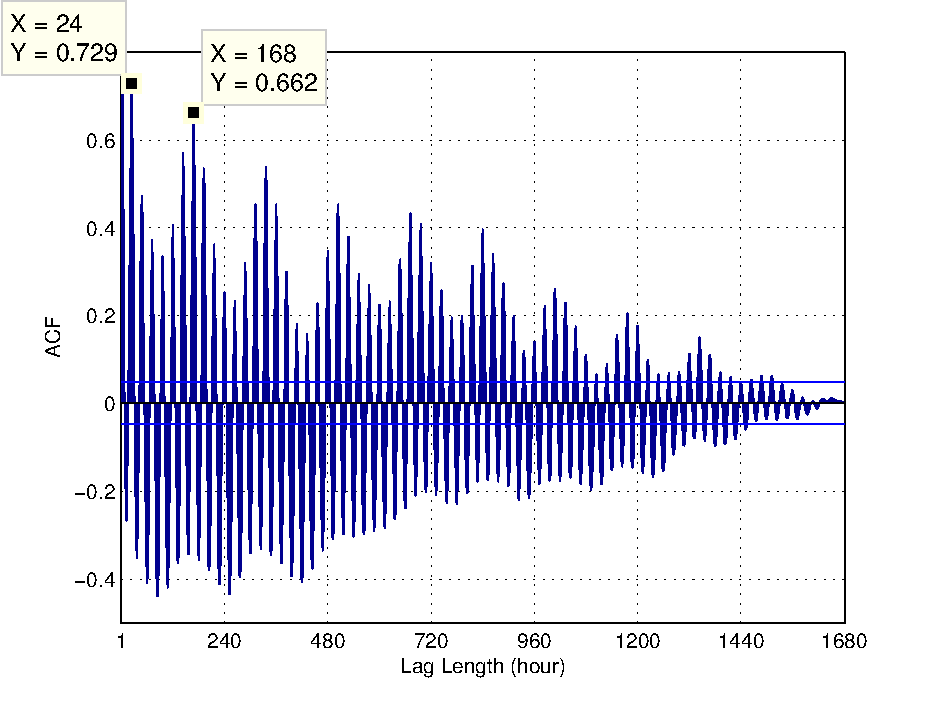
\includegraphics[width=.45\textwidth]{img/acf_101A1_GHP-eps-converted-to.pdf}
\caption{Auto-correlation of a usual signal from the Engineering Building 2 dataset.
The signal features daily and weekly patterns (resp. $x=24$ and $x=168$).}
\label{fig:autocorr}
\end{center}
\end{figure}

Intuitively the dominant pattern driven by office hours is responsible for these unexpected results.
As shown in Figure \ref{fig:diagram1} the two 1-week long raw signals feature the same dominant pattern that hides the signal smaller fluctuations providing details of the devices usage.

Indeed, thorough inspection of the data reveals that the correlation metric is insufficient with raw signals containing the same dominant pattern.
Our data inspection uncovered a few dominant patterns common to building energy consumption data \cite{wrinch:pes2012}.
Figure \ref{fig:autocorr} depicts the auto-correlation of a usual electricity consumption signal.
The two highest values in the figure correspond to a lag of 24 hours and 168 hours (one week) meaning that the signal is clearly periodic and similar data reappears every day/week.
The daily pattern stands out due to office hours whereas the weekly pattern correspond to the distinct power consumption during weekdays and weekends.

One of the major challenge in this work is to discard these patterns and uncover devices intrinsic relationships.
This difficulty is overcome by the first part of the method (Strip and Bind) presented in Section \ref{methodo:est}.
Then, the second part of the method (Search) monitors over time the devices relationships and detect abnormal device behavior changes (Section \ref{methodo:ano}).
